Aubrey tiene un nuevo estuche de arte con forma de prisma rectangular.
El estuche es de 12 cm$^3$. Lo único dentro del estuche es un nuevo borrador rosa con las dimensiones
como se muestran en la figura \ref{fig:vol_area_03}.

\textbf{¿Cuál es el volumen del estuche que no ocupa por el borrador?}\\

\begin{minipage}{0.3\linewidth}
    \begin{figure}[H]
        \begin{center}
            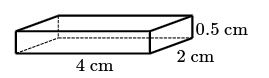
\includegraphics[width=1\textwidth]{../images/vol_area_03}
        \end{center}
        \caption{}
        \label{fig:vol_area_03}
    \end{figure}
\end{minipage}
\begin{minipage}{0.7\linewidth}
    \begin{solutionbox}{3cm}
        Si restamos el volumen del borrador  al volumen del estuche, entonces podremos conocer el espacio que no es ocupado por el borrador, así:
        \[12 \text{cm}^3 - \left(4 \text{ cm} \times 2 \text{ cm} \times 0.5 \text{ cm}\right)=12 \text{ cm}^3 - 4 \text{ cm}^3 = 8 \text{cm}^3   \]
    \end{solutionbox}
\end{minipage}